\section{Introduction}

Power law distributions in Nature usually signal the absence of a
scale in the region where the scaling is observed, and sometimes point
to critical dynamics. In Self-Organized-Criticality (SOC)
\citep{BTW87,BTW88}, for example, power law distributions reveal the
dynamics of an unstable critical point, brought about by slow driving
and a feed-back mechanism between order parameter and critical
parameter.  The critical dynamics is usually described within the
language of second-order phase transitions in condensed matter systems
\citep{SJD}, but it can be shown that SOC-type behavior also occurs
within a dual description in terms of the Landau-Ginzburg equation as
{\em first-order} transitions \citep{GS}.  Indeed, it was shown that a
power law distribution of {\em epoch-lengths}, that is, the time a
particular species dominates the dynamics of an adapting population,
is explained by a self-organized critical scenario \citep{CA2} that
carries the hallmark of first-order phase transitions. Here, we
measure the distribution of abundances of {\em species} and genotypes
in an artificial chemistry, \citep[the Avida Artificial Life
system][]{AB1,OBA} and show that the distribution is scale-free under
a broad class of circumstances, confirming the results reported in
\citep{CA2}.  In the next section, we discuss the first-order dynamics
in more detail and examine ``avalanches of invention'' from the point
of view of a thermodynamics of information. In Section III, we measure
the critical exponent of the power law of genotype abundances in the
limit of infinitesimal driving, i.e., infinitesimal mutation rate, and
discuss the role of the fitness landscape in shaping the
distribution. In Section IV, we repeat the analysis for a higher
taxonomic level (that of species) and discuss its relation to the
geometric distributions found by \citet{BUR90,BUR93}.
Conclusions about the evolutionary process drawn from the data
obtained in this paper are presented in Section V.

\begin{figure}[t]
\begin{center}
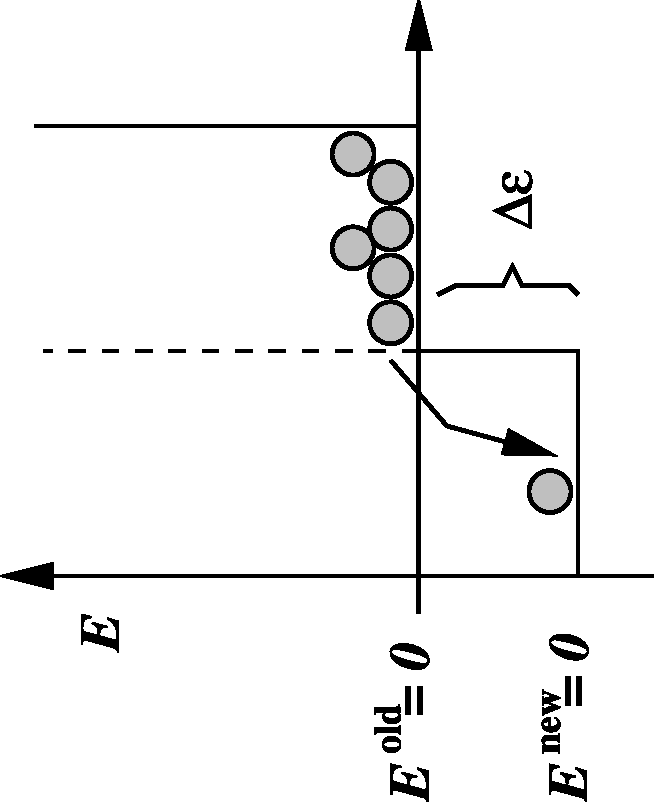
\includegraphics[width=2.1in,angle=-90]{img/fig1}
\caption{``Energies'' (inferiorities) of strings in a first-order
  phase transition with latent heat $\Delta\epsilon$.}
\label{fig1}
\end{center}
\end{figure}

